\documentclass[twocolumn]{article}
\usepackage{amsmath}
\usepackage{amssymb}
\usepackage{graphicx}
\usepackage{cite}
\bibliographystyle{plain}
\usepackage[numbers]{natbib}

\title{Belleza Matemática: Explorando la Estética en los Conceptos Numéricos}
\author{Brenda Vargas Parra}
\date{}

\begin{document}

\maketitle


La belleza ha sido asociada con el arte, la música y la literatura, disciplinas en las que la estética juega un papel central, sin embargo, veremos cómo esta noción también se extiende a las matemáticas, donde ciertas ecuaciones, teoremas y patrones han sido considerados bellos por matemáticos y filósofos a lo largo del tiempo. Un ejemplo icónico es la identidad de Euler, llamada incluso "una de las ecuaciones más hermosas de las matemáticas"

\begin{equation}
    e^{i\pi} + 1 = 0
\end{equation}



Esta ecuación es admirada por su simplicidad y la forma en que relacionan cinco constantes fundamentales: $e$, $i$, $\pi$, 1 y 0 \cite{hardy1940}. Para conocedores, este tipo de relaciones provocan armonía y elegancia similar a la que se experimenta al contemplar una obra de arte.


\begin{figure}[h]
    \centering
    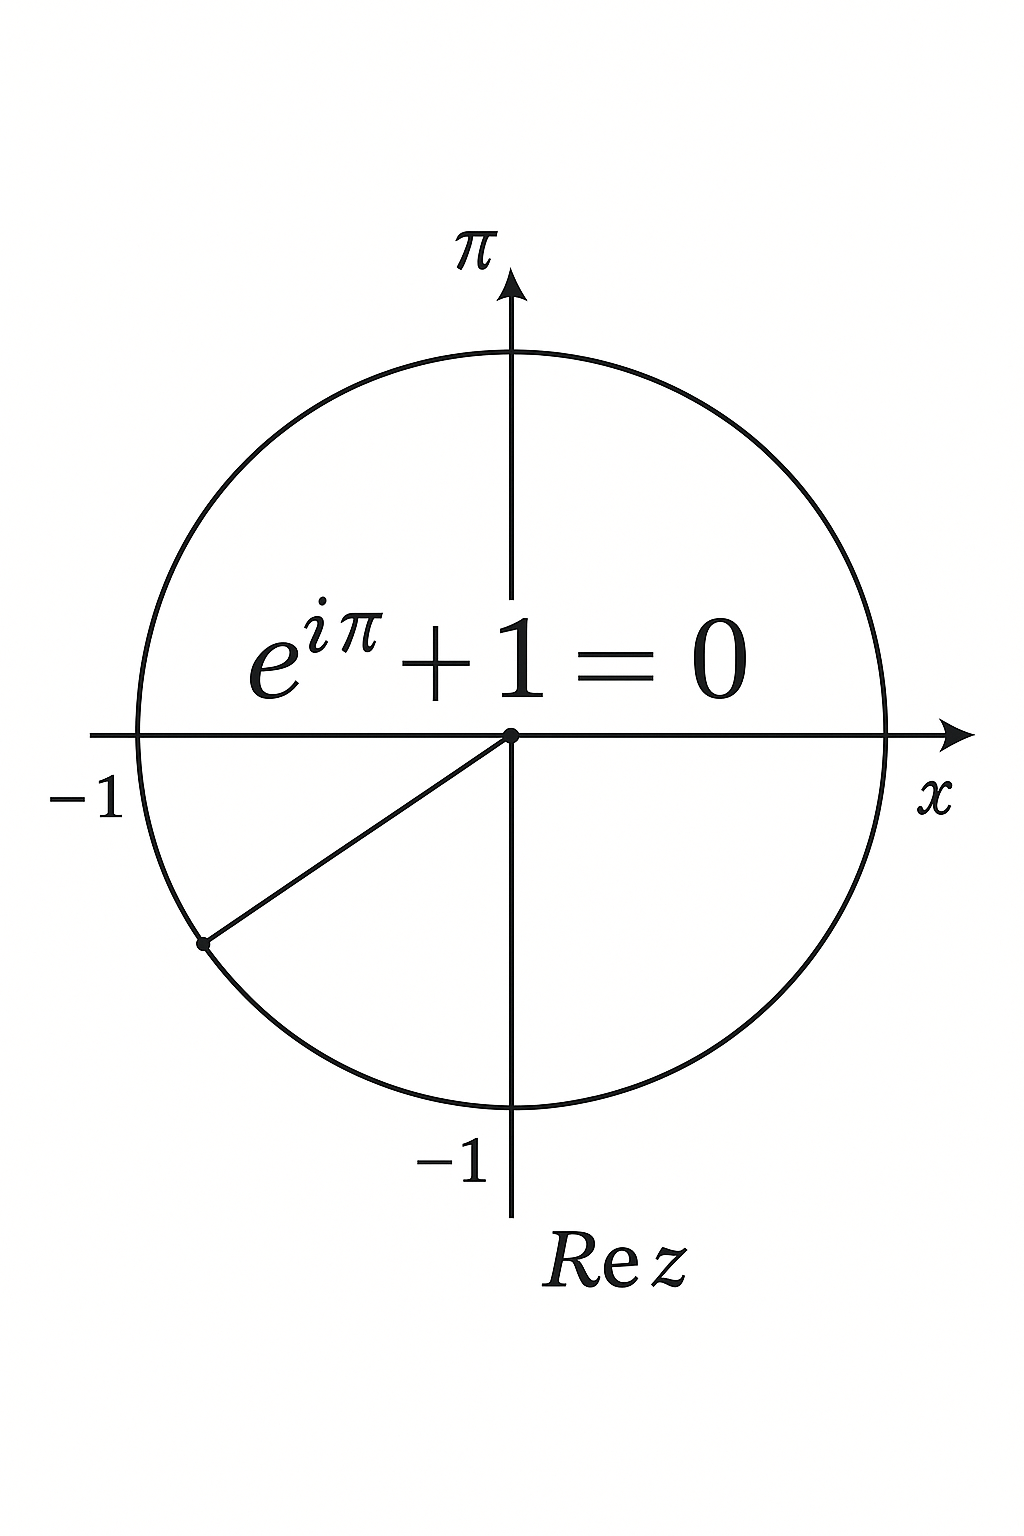
\includegraphics[width=0.5\linewidth]{imagen2.png}
    \caption{Representación geométrica de la identidad de Euler}
    \label{fig:enter-label}
\end{figure}

A continuación se analizará la existencia de la belleza en las matemáticas. Se explorará cómo los matemáticos caracterizan dicha belleza, si esta noción es subjetiva o tiene bases objetivas, y en qué medida es comparable a la belleza en el arte. Para ello, se abordarán antecedentes históricos, opiniones de matemáticos y filósofos, así como ejemplos concretos de conceptos matemáticos que han sido descritos como bellos.

En este análisis se estructura la definición de belleza matemática (formal y subjetivamente), para posteriormente, comparar la belleza en la matemática con la del arte y ver que tan similares son. 


Empecemos con la noción de belleza, la cual ha sido objeto de reflexión filosófica desde la antigüedad, se encuentra que Platón la asociaba con la armonía y el orden en su teoría de las formas, mientras que Aristóteles enfatizaba la proporción y la simetría en su estudio de la estética \cite{platon_republic, aristoteles_poetica}. A hoy podemos tener una perspectiva distinta.

La belleza en general se define como una cualidad que genera placer estético o admiración en quien la percibe. Esta percepción puede depender de factores cognitivos, emocionales y sensoriales \cite{tatarkiewicz2005}. con distintos tipos de naturaleza:

\begin{itemize}
    \item \textbf{Teoría objetiva:} Defiende que la belleza es una propiedad inherente a los objetos, basada en cualidades como la proporción, la simetría y la armonía \cite{eco1987}.
    \item \textbf{Teoría subjetiva:} Sostiene que la belleza depende de la percepción individual y la experiencia del observador \cite{kant1790}.
    \item \textbf{Teoría funcionalista:} Considera que la belleza está relacionada con la eficacia y la adecuación de una estructura para cumplir un propósito \cite{gombrich1969}.
\end{itemize}


\vspace{3}

 
 Hermann y Hardy argumentan ciertas propiedades estructurales, como la simetría, la elegancia y la simplicidad, propias de la naturaleza objetiva, que hacen que una fórmula o teorema sea intrínsecamente bello \cite{hardy1940, weyl1952}. Por otra parte Sinclair la ve como subjetiva ya que sostiene que la belleza matemática depende de la percepción y la intuición del matemático, influenciada por factores culturales y emocionales \cite{sinclair2006}. Pero Gian-Carlo Rota, matemático y filósofo fallecido en 1999 argumentaba que la belleza matemática está relacionada con la inevitabilidad, es decir, cuando una demostración parece ser la única manera "natural" de llegar a un resultado, se percibe como bella \cite{rota1997}. Se podría suponer que la belleza en matemáticas surge cuando un resultado parece evidente y adecuado en retrospectiva.

Es así que desde este punto, se observan diferentes autores quienes han identificado principios esenciales que rigen la belleza en matemáticas.

\texttt{Simplicidad:} Los resultados matemáticos bellos suelen tener una forma compacta y fácil de entender. Hardy defendía que una demostración matemática elegante es aquella que evita pasos innecesarios y revela la esencia del problema de manera clara \cite{hardy1940}.
    
\texttt{Simetría:} La presencia de estructuras simétricas en fórmulas y teoremas es considerada un rasgo estético fundamental. Weyl sostiene que la simetría es la base de muchas manifestaciones de belleza en matemáticas, desde los grupos algebraicos hasta las ecuaciones físicas \cite{weyl1952}.

\begin{figure} [h]
    \centering
    
\includegraphics[width=0.5\linewidth]{imagen3.png}
    \caption{copo de nieve con estructura fractal}
    \label{fig:enter-label}
\end{figure}
    
\texttt{Profundidad:} Un resultado matemático es bello cuando tiene implicaciones inesperadas o conecta con otras áreas del conocimiento. Steiner argumenta que la belleza matemática radica en su capacidad de revelar verdades profundas de manera accesible \cite{steiner2001}.
    
\texttt{Sorpresa:} La belleza también surge cuando un resultado es inesperado pero, una vez comprendido, parece obvio. Esto se observa en teoremas como el de los números primos gemelos o en la identidad de Euler \cite{francis2015}.
    
\texttt{Aplicabilidad:} La belleza de las matemáticas se encuentra también en su capacidad de describir el mundo físico con precisión. La ecuación de onda y las ecuaciones de Maxwell son ejemplos de cómo estructuras matemáticas elegantes explican fenómenos de la naturaleza \cite{livio2017}.


Hasta ahora, hemos explorado la belleza matemática desde una perspectiva objetiva, identificando propiedades intrínsecas como la simetría, la simplicidad y la elegancia. Sin embargo, la apreciación de la belleza matemática no es universal ni estática; depende de la percepción, la intuición y la experiencia del observador. 

Según Sinclair, la belleza matemática es una experiencia subjetiva que varía entre matemáticos y culturas \cite{sinclair2006}. Lo que un matemático encuentra bello puede no tener el mismo impacto en otro, debido a diferencias en formación, contexto y sensibilidad estética. Por ejemplo, un estudiante que por primera vez descubre el triángulo de Pascal podría llegar a  experimentar asombro por los patrones emergentes, mientras que un matemático experimentado podría ver belleza en sus conexiones con combinatoria, teoría de números y probabilidad.

\begin{figure}
    \centering
    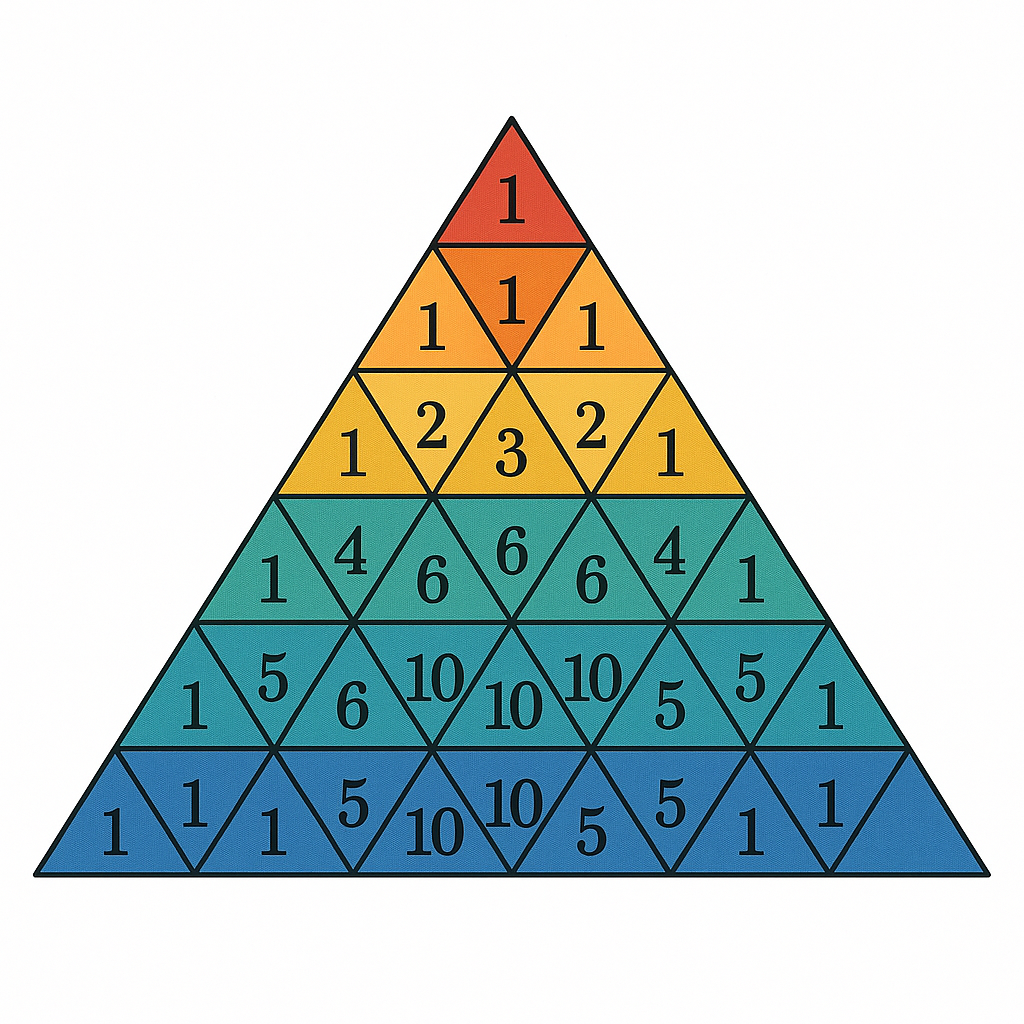
\includegraphics[width=0.5\linewidth]{imagen4.png}
    \caption{Triángulo de Pascal}
    \label{fig:enter-label}
\end{figure}


La belleza matemática no solo se manifiesta en la estructura formal de un teorema, sino también en la experiencia emocional individual. Hardy menciona que un resultado matemático bello produce una sensación de satisfacción y admiración, comparable a la contemplación de una obra de arte \cite{hardy1940}. De manera similar, Poincaré describe cómo las ideas matemáticas surgen de la intuición y generan una sensación de armonía antes de ser formalizadas \cite{poincare1913}.

Para muchos matemáticos, la belleza radica en la sensación de haber encontrado una "verdad inevitable". Gian-Carlo Rota sugiere que la belleza matemática se percibe cuando una solución parece la única posible, como si la naturaleza misma dictara el resultado \cite{rota1997}. Esta apreciación estética puede variar de persona a persona, dependiendo del proceso de aprendizaje individual.

Dado que la percepción de belleza para la naturaleza subjetiva depende cada quien, también puede estar influenciada por el contexto cultural, por ejemplo en la Grecia antigua la belleza se asociaba con la demostración geométrica y la armonía de las proporciones, como se observa en los sólidos platónicos. En la matemática china y árabe, se enfatizaban patrones y simetrías en álgebra y teoría de números.Pero actualmente, la belleza se aprecia en la abstracción y la unificación de teorías aparentemente dispares, como la relación entre el álgebra y la geometría en la teoría de grupos.

Mientras que algunos matemáticos encuentran belleza en la rigurosidad formal, otros la perciben en la intuición y la creatividad del proceso matemático. Pero ¿se puede comparar la belleza artística con la "belleza matemática"?

La belleza ha sido un concepto central tanto en las matemáticas como en el arte. Desde hace mucho se ha observado que ciertas estructuras, proporciones y patrones generan una sensación de armonía y elegancia, independientemente de su campo de aplicación. Pero, ¿es la belleza en la matemática equivalente a la belleza en el arte?

 Mientras que en el arte la belleza suele asociarse con la creatividad, la expresión subjetiva y la emoción, en matemáticas se encuentra en la estructura, la simplicidad y la precisión \cite{livio2017}. Sin embargo, en ambos casos, se percibe el asombro, admiración y una sensación de descubrimiento.

A continuación, las similitudes y diferencias entre la belleza matemática y la artística.

Tanto en matemáticas como en el arte importa la presencia de orden y simetría. La simetría es una propiedad esencial en geometría, álgebra y física, y se manifiesta en muchas estructuras artísticas, desde la arquitectura clásica hasta la pintura renacentista \cite{weyl1952}. 

Un ejemplo icónico es el uso de la \textit{}{proporción áurea}, representada por el número irracional:

\begin{equation}
    \varphi = \frac{1 + \sqrt{5}}{2} \approx 1.618
\end{equation}

Esta proporción se encuentra en estructuras naturales como conchas de nautilus, en composiciones artísticas como La Gioconda de Leonardo da Vinci y en la arquitectura del Partenón de Atenas \cite{livio2002}. En matemáticas, la proporción áurea también aparece en la sucesión de Fibonacci y en estructuras fractales \cite{livio2017}.


\begin{figure} [h]
    \centering
    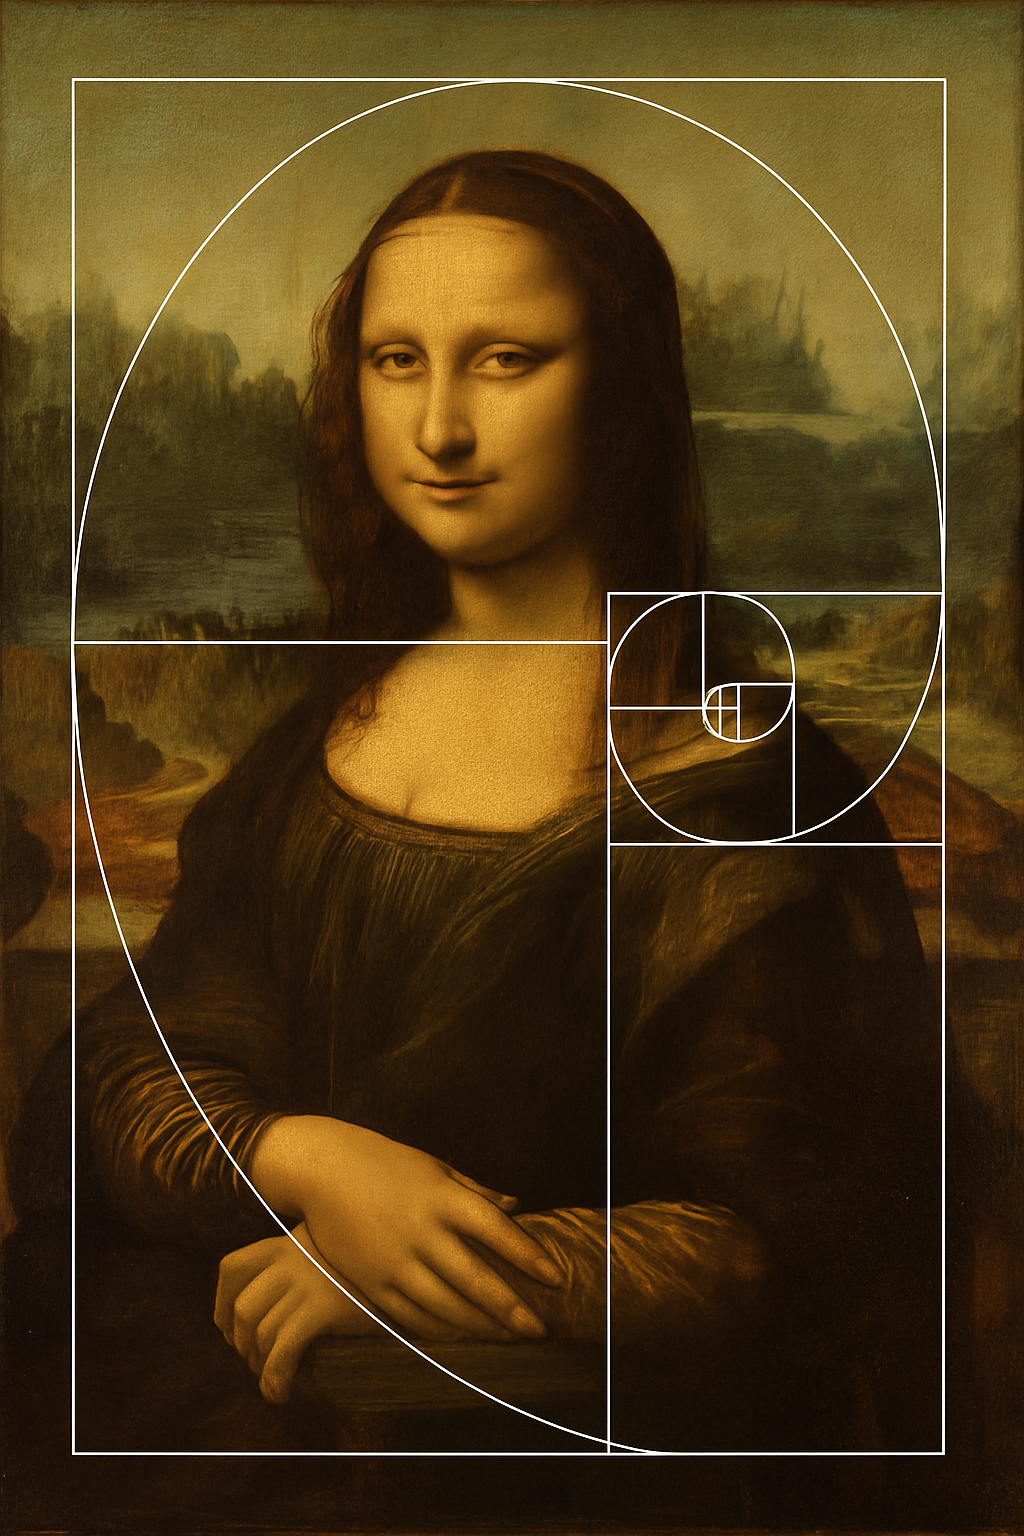
\includegraphics[width=0.5\linewidth]{imagen5.png}
    \caption{Proporción áurea en La Gioconda}
    \label{fig:enter-label}
\end{figure}


La belleza en ambas disciplinas se relaciona con la simplicidad y la elegancia. Una ecuación matemática es más bella cuando expresa una idea profunda con el menor número de elementos posibles, de manera similar a cómo una obra de arte minimalista puede transmitir emociones con pocos recursos. 

Hardy argumentaba que una demostración matemática es hermosa cuando es directa, clara y sin pasos innecesarios \cite{hardy1940}. De la misma manera, en la pintura y la escultura, las formas más simples pueden generar un impacto visual fuerte, como en las obras de Piet Mondrian o en la escultura moderna de Brâncuși.

\subsubsection{Sorpresa y Creatividad}

Tanto en el arte como en la matemática, la \textbf{belleza puede surgir de lo inesperado}. En matemáticas, algunos resultados como la identidad de Euler:

\begin{equation}
    e^{i\pi} + 1 = 0
\end{equation}

son considerados bellos no solo por su estructura, sino también porque conectan elementos aparentemente independientes en una relación profunda e inesperada \cite{francis2015}. En el arte, movimientos como el surrealismo han utilizado lo inesperado para crear obras visualmente impactantes, desafiando las expectativas del espectador.

\subsubsection{Emoción y Estética}

Aunque a menudo se considera que las matemáticas son puramente racionales y el arte es subjetivo, ambos pueden generar una respuesta emocional en quienes los aprecian. La contemplación de una demostración elegante o de una pintura bien compuesta puede evocar asombro y admiración. Como señala Sinclair, la experiencia estética en matemáticas no solo se basa en su estructura lógica, sino también en la intuición y la emoción del matemático \cite{sinclair2006}.

\section*{Conclusión}

La belleza matemática, muy pero muy lejos de ser un concepto netamente para el uso de quienes dominan el lenguaje numérico, se vislumbra como una experiencia estética que trasciende lo lógico o racional. A lo largo de este ensayo, se observó que la belleza en las matemáticas puede surgir tanto de cualidades objetivas como la simetría, la simplicidad y la elegancia, como de apreciaciones subjetivas ligadas a la intuición, la sorpresa y la emoción.

Al igual que en el arte, la belleza matemática despierta admiración y asombro, aunque sus caminos hacia esa experiencia difieran: mientras el arte se nutre de la expresión creativa y emocional, las matemáticas encuentran belleza en la estructura, la precisión y la conexión inesperada entre conceptos. Esta dualidad permite entender que la belleza no pertenece a una sola disciplina, sino que es un puente entre la lógica y la sensibilidad humana.

Comprender la belleza matemática no solo amplía nuestra visión del conocimiento, sino que también nos invita a apreciar la creatividad inherente al pensamiento abstracto. Al final, tanto en una obra de arte como en una ecuación elegante, lo que se manifiesta es la capacidad del ser humano para encontrar armonía en el mundo que lo rodea.


\bibliography{bibliografia}
\end{document}
